
\documentclass[a4paper]{scrreprt}
 
\usepackage[german]{babel}
\usepackage[utf8]{inputenc}
\usepackage[T1]{fontenc}
\usepackage{ae}

\usepackage[scaled]{helvet}
\renewcommand\familydefault{\sfdefault} 

\usepackage[onehalfspacing]{setspace}
\usepackage[scaled]{helvet}
\renewcommand*\familydefault{\sfdefault}

\usepackage[T1]{fontenc}
\usepackage{glossaries}
\usepackage{graphicx}
\usepackage[bookmarks,bookmarksnumbered]{hyperref}
\usepackage{float}
\usepackage[font={footnotesize}]{caption}

\setcounter{tocdepth}{1} 
\setcounter{secnumdepth}{2} 

\makenoidxglossaries

\newglossaryentry{Server}
{	name=Server,
	description={Ein Server (englisch server, wörtlich Diener oder Bediensteter, im weiteren Sinn auch Dienst) ist ein Computerprogramm oder ein Computer, der Computerfunktionalitäten wie Dienstprogramme, Daten oder andere Ressourcen bereitstellt, damit andere Computer oder Programme („Clients“) darauf zugreifen können}
}

\newglossaryentry{App}
{ 	name=App,
	plural=Apps,
	description={Als Mobile App (auf Deutsch meist in der Kurzform die App, eine Abkürzung für den Fachbegriff Applikation) wird eine Anwendungssoftware für Mobilgeräte beziehungsweise mobile Betriebssysteme bezeichnet}
}

\newglossaryentry{Nutzer}
{	name=Nutzer,
	description={Ein Benutzer (auch Endbenutzer, Bediener oder kurz Nutzer genannt sowie englisch User) ist eine Person, die ein Hilfs- oder Arbeitsmittel zur Erzielung eines Nutzens verwendet, beispielsweise für eine Zeitersparnis oder Kostensenkung}
}

\newglossaryentry{Desktop Anwendung}
{	name=Desktop Anwendung,
	plural=Desktop Anwendungen,
	description={Als Desktop Anwendungen (auch Anwendungsprogramm, kurz Anwendung oder Applikation; englisch application software, kurz App) werden Computerprogramme bezeichnet, die genutzt werden, um eine nützliche oder gewünschte nicht systemtechnische Funktionalität zu bearbeiten oder zu unterstützen. Sie dienen der „Lösung von Benutzerproblemen“}
}

\newglossaryentry{Drag and Drop}
{	name=Drag and Drop,
	description={Drag and Drop, oft auch Drag’n’Drop, deutsch „Ziehen und Ablegen“, ist eine Methode zur Bedienung grafischer Benutzeroberflächen von Rechnern durch das Bewegen grafischer Elemente mittels eines Zeigegerätes. Ein Element wie z. B. ein Piktogramm kann damit gezogen und über einem möglichen Ziel losgelassen werden. Dieses kann zum Beispiel markierter Text oder das Symbol einer Datei sein }
}

\newglossaryentry{Medikament}
{	name=Medikament,
	description={Arzneimittel oder gleichbedeutend Medikamente (lateinisch medicamentum „Heilmittel“) sind Stoffe oder Stoffzusammensetzungen, die „zur Heilung oder zur Verhütung menschlicher oder tierischer Krankheiten bestimmt sind“ oder sich dazu eignen, physiologische Funktionen zu beeinflussen oder eine medizinische Diagnose zu ermöglichen}
}

\newglossaryentry{NFC}
{ 	name=NFC,
	description={Die Nahfeldkommunikation (Near Field Communication, abgekürzt NFC) ist ein auf der RFID-Technik basierender internationaler Übertragungsstandard zum kontaktlosen Austausch von Daten per elektromagnetischer Induktion mittels loser gekoppelter Spulen über kurze Strecken von wenigen Zentimetern}
}

\newglossaryentry{Versichertennummer}
{ 	name=Versichertennummer,
	description={Die Krankenversichertennummer dient der Identifikation des Versicherten bei einer Krankenversicherung. Die Krankenversichertennummer wird benötigt, damit Leistungserbringer, z. B. Ärzte oder Zahnärzte ihre Leistungen mittels der Krankenversicherungskarte, über die Kassenärztlichen Vereinigungen, mit der zuständigen Krankenkasse abrechnen können}
}


\newglossaryentry{Bluetooth}
{	name=Bluetooth,
	description={Bluetooth ist ein in den 1990er Jahren durch die Bluetooth Special Interest Group (SIG) entwickelter Industriestandard gemäß IEEE 802.15.1 für die Datenübertragung zwischen Geräten über kurze Distanz per Funktechnik (WPAN). Dabei sind verbindungslose sowie verbindungsbehaftete Übertragungen von Punkt zu Punkt und Ad-hoc- oder Piconetze möglich}
}

\newglossaryentry{Pop-Up}
{	name=Pop-Up,
	description={Ein Pop-up (von englisch to pop up, „plötzlich auftauchen“) ist ein Element einer grafischen Benutzeroberfläche. In der Regel werden Pop-ups eingesetzt, um zusätzliche Inhalte anzuzeigen oder eine bestimmte Interaktion abzufragen. Typischerweise „springen“ Pop-ups auf und überdecken dabei andere Teile der Benutzeroberfläche}
}

\newglossaryentry{Cloud}
{	name=Cloud,
	description={Die Cloud ist keine physische Größe, sondern ein riesiges Netzwerk aus Remoteservern, die über die ganzen Welt verteilt aber miteinander verbunden sind, damit sie als ein einziges großes Ökosystem funktionieren können}
}

\newglossaryentry{Tab}
{	name=Tab,
	description={Eine Registerkarte, auch Reiter oder Tab genannt, ist ein Steuerelement einer grafischen Benutzeroberfläche, das einem Registerblatt aus Aktenschränken nachempfunden wurde }
}
 
\newglossaryentry{Arztbrief}
{	name=Arztbrief,
	plural=Arztbriefe,
	description={Der Arztbrief, oft synonym als Epikrise, Entlassungsbrief, Patientenbrief oder Befundbericht bezeichnet, ist ein Transferdokument für die Kommunikation zwischen Ärzten. Der Arztbrief gibt einen zusammenfassenden Überblick über den Status des Patienten bei der Entlassung, einen Rückblick über den Krankheitsverlauf, die veranlasste Therapie, eine Interpretation des Geschehens zum Krankheitsverlauf im speziellen Fall}
}

\newglossaryentry{Anamnese}
{	name=Anamnese,
	description={Die Anamnese (von altgriechisch anámnēsis, deutsch ‚Erinnerung‘) ist die professionelle Erfragung von potenziell medizinisch relevanten Informationen durch Fachpersonal (z. B. einen Arzt)}
}
 
\begin{document}
\begin{titlepage}
\begin{figure}[h]
	\vspace{-4cm}
	\hspace{-2cm}
	
\includegraphics[ width=0.3\textwidth]{Kit_Logo}
	\label{fig:Aufg03_1}
\end{figure}
	\vspace{1.5cm}
	\centering
	
\includegraphics[width=0.5\textwidth]{graphics/myMD_Logo}\par\vspace{0.5cm}
	{\Huge myMD \par}
	\vspace{2cm}
	{\scshape\Large Entwurf\par}
	\vspace{1cm}
	Praxis der Softwareentwicklung WS2017/2018 \par
	\vspace{2cm}
	{\Large\itshape Philipp Pelcz, Philipp Karcher, Jan-Luca Vettel\par}
	\vfill
	supervised by \par
	Marc Aurel Kiefer

	\vfill

% Bottom of the page
	{\large \today \par}
\end{titlepage}
 

% Platzierung des Inhaltsverzeichnisses
\tableofcontents
\addtocontents{toc}{\protect\enlargethispage{10cm}}



\chapter{Zielbestimmung}

\section{Einleitung}
Die digitale Vernetzung aller Lebensbereich dominiert und verändert unseren Alltag seit einigen Jahren wie kaum eine andere Thematik. Viele Branchen erfahren eine sogenannte „digitale Transformation“, die industrielle Produktion soll mittels Industrie 4.0 in das Zeitalter moderner Informationstechnik befördert werden und dank des „Internet der Dinge“ (Internet of Things) kommuniziert eine stetig wachsende Zahl an Alltagsgegenständen über das Internet untereinander, mit dem Ziel, uns das Leben zu erleichtern.\\
Mit dem „E-Health-Gesetz“ hat die Bundesregierung im Jahr 2016 einen Vorstoß unternommen, die digitale Infrastruktur im Gesundheitswesen auszubauen, um so eine der größten Branchen der deutschen Wirtschaft zu digitalisieren.\\
Tatsächlich reicht ein kurzer Blick in die meisten deutschen Arztpraxen oder Krankenhäuser aus, um festzustellen, dass auch heute noch Papier als Speichermedium der Wahl eingesetzt wird. Wenngleich eine große Zahl an Praxen und Kliniken mittlerweile Software zur internen Datenverwaltung einsetzt, so erfolgt die Kommunikation mit dem Patient in den wenigsten Einrichtungen digital.\\
~\\
Im Rahmen der Veranstaltung „Praxis der Softwareentwicklung (PSE)“ und des „Imagine Cup 2018“, einem von Microsoft veranstalteten Wettbewerb, hat es sich unser Team zum Ziel gemacht, dies zu ändern:\\
Mit der Entwicklung von myMD soll es dem Arzt künftig möglich sein, einem Patienten die ihn betreffenden Arztbriefe und Krankenakten in digitaler Form noch im Behandlungszimmer aushändigen zu können. 
Zur selben Zeit ermöglicht myMD es dem Patienten, all seine Patientendaten, Arztbriefe und Krankenakten, die bisher verstreut auf den Computern dutzender Ärzte gesichert waren, an einem Ort zentral gespeichert auf seinem Mobilgerät immer unter Kontrolle zu haben. 

\newpage
Die Möglichkeiten, die solch ein System Ärzten und Patienten gleichermaßen bieten könnte, reichen von einer naheliegenden Reduktion des Papierverbrauchs in Arztpraxen und Krankenhäusern bis hin zu einer möglichen Minderung gefährlicher Medikamentenwechselwirkungen, an denen jährlich alleine in Deutschland mehrere Zehntausend Menschen sterben.\\
Der Arzt wäre beispielsweise bei der \gls{Anamnese} nicht alleine auf das Erinnerungsvermögen des Patienten angewiesen, sondern könnte sich mit wenigen Handgriffen ein vollständiges Bild über die Krankengeschichte verschaffen, mögliche Unverträglichkeiten in Erfahrung bringen und aktuelle oder vergangene Medikamenteneinnahmen studieren, die sich unter Umständen auf die eigene Diagnose und Therapieempfehlung auswirken könnten.\\
Gleichzeitig könnte myMD den Patienten besser vor überflüssigen Mehrfachuntersuchungen und somit beispielsweise unnötiger Strahlenbelastung schützen, da der Nutzer zu jeder Zeit alle Befunde und Untersuchungsergebnisse auf dem eigenen Mobilgerät bei sich trägt. Ein weiterer wichtiger Aspekt ist hierbei die zeitlich unbegrenzte Archivierung der gespeicherten Gesundheitsinformationen, denn im Gegensatz zur gesetzlich vorgeschriebenen Mindestspeicherdauer von 10 Jahren kann der Patient mit myMD selbst entscheiden, ob und wann er Einträge von seinem Mobilgerät entfernen möchte. Gerade für Krebspatienten, die neben der Datenvollständigkeit häufig auch mit enormen Papier- und Aktenbergen zu kämpfen haben, wäre dies eine hilfreiche Unterstützung.\\

Betont werden sollte auch, dass mit der 2018 in Kraft tretenden EU-Datenschutz-\\Grundverordnung (EU-DSGVO, §20 "Recht auf Datenübertragbarkeit") dem Verbraucher, sprich dem Patienten, das Recht eingeräumt wird, die bei einem Arzt (Dienstleister) anfallenden, sie selbst betreffenden Daten in einem gängigen, maschinenlesbaren Format erhalten zu können. Mit dem Einsatz von myMD könnte ein Arzt dieser rechtlichen Anforderung mühelos nachkommen.\\

Insgesamt ist es unser erklärtes Ziel, durch myMD die Vorgänge in Arztpraxen und Klinken aus der Sicht der Patienten transparenter zu gestalten und dem Patienten durch die strukturierte Darstellung seiner gesamten Krankenhistorie eine umfassende Übersicht über den eigenen Gesundheitsverlauf zu verschaffen.

 
\section{Pflichtkriterien (PK)}
\subsection{Patientenseitige Datenübertragung}
\begin{tabular}{lll}

[PK1010] & \multicolumn{2}{p{12cm}}  {\glspl{Arztbrief} können von der \gls{Desktop Anwendung} auf die myMD \gls{App} des Patienten übertragen werden.} \\
{[PK1020]} & \multicolumn{2}{p{12cm}}  {Die Übertragung erfolgt verschlüsselt über \gls{Bluetooth}.} \\
{[PK1030]} & \multicolumn{2}{p{12cm}}  {Eine laufende Datenübertragung kann manuell abgebrochen werden.} \\

\end{tabular}

\subsection{Darstellung}
\begin{tabular}{lll}
[PK2010] & \multicolumn{2}{p{12cm}}  {\glspl{Arztbrief} werden chronologisch absteigend im \gls{Tab} \textit{Übersicht} dargestellt.} \\
{[PK2020]} & \multicolumn{2}{p{12cm}}  {Der \gls{Nutzer} kann überflüssige/unerwünschte \glspl{Arztbrief} löschen.} \\
{[PK2030]} & \multicolumn{2}{p{12cm}}  {Die Darstellung eines Arztbriefes umfasst die Diagnose, verordnete \gls{Medikament}e, das Datum und den Namen des behandelnden Arztes.} \\
\end{tabular}

\subsection{Einstellungen}
\begin{tabular}{lll}
[PK3010] & \multicolumn{2}{p{12cm}}  {Der \gls{Nutzer} kann ein eigenes Profil anlegen, welches Daten wie den Namen, Versicherungsnummer, Blutgruppe und Allergien enthält.} \\
{[PK3020]} & \multicolumn{2}{p{12cm}}  {Die myMD \gls{App} wird in Deutsch angeboten.} \\

\end{tabular}

\subsection{\gls{Desktop Anwendung}}
\begin{tabular}{lll}
{[PK4010]} & \multicolumn{2}{p{12cm}}  {Die \gls{Desktop Anwendung} kann die Geräte in der Nähe anzeigen.} \\
{[PK4020]} & \multicolumn{2}{p{12cm}}  {Der Arzt kann unter den Geräten in der Nähe das Mobilgerät des Patienten als Empfänger auswählen.} \\
{[PK4030]} & \multicolumn{2}{p{12cm}}  {Digitale \glspl{Arztbrief} können entweder per \gls{Drag and Drop} oder über einen Explorer in die \gls{Desktop Anwendung} geladen werden.} \\
{[PK4040]} & \multicolumn{2}{p{12cm}}  {Die Daten werden auf Knopfdruck an das Mobilgerät des Patienten gesendet.} \\
\end{tabular}

\subsection{Kompatibilität}
\begin{tabular}{lll}
[PK5010] & \multicolumn{2}{p{12cm}}  {Die \gls{Desktop Anwendung} wird von Microsoft Windows 10 unterstützt.} \\
{[PK5020]} & \multicolumn{2}{p{12cm}}  {Die myMD \gls{App} wird von Android 6.0 (und höher) unterstützt.} \\
{[PK5030]} & \multicolumn{2}{p{12cm}}  {Die myMD \gls{App} kann \glspl{Arztbrief} im .hl7 Dateiformat anzeigen.} \\

\end{tabular}
 
\section{Wunschkriterien (WK)}
\subsection{Patientenseitige Datenübertragung}
\begin{tabular}{lll}
[WK1010] & \multicolumn{2}{p{12cm}}  {Ein \gls{Arztbrief} kann von der myMD \gls{App} des Patienten auf die \gls{Desktop Anwendung} übertragen werden.} \\
{[WK1020]} & \multicolumn{2}{p{12cm}}  {Der Patient kann mehrere \glspl{Arztbrief} gleichzeitig senden.} \\
{[WK1030]} & \multicolumn{2}{p{12cm}}  {\gls{NFC} steht als weitere Übertragungsmöglichkeit zur Verfügung.} \\
{[WK1040]} & \multicolumn{2}{p{12cm}}  {Der Patient wird vor dem Senden von sensiblen Daten darauf hingewiesen, dass er sensible Daten versendet.} \\
{[WK1050]} & \multicolumn{2}{p{12cm}}  {Ein Profil auf einem Mobilgerät kann auf ein anderes übertragen werden.} \\

\end{tabular}

\subsection{Darstellung}
\begin{tabular}{lll}
[WK2010] & \multicolumn{2}{p{12cm}}  {Eingenommene \gls{Medikament}e werden in einem extra \gls{Tab} chronologisch absteigend sortiert dargestellt.} \\
{[WK2020]} & \multicolumn{2}{p{12cm}}  {Laborwerte des Patienten werden in einem extra \gls{Tab} chronologisch absteigend sortiert dargestellt.} \\
{[WK2030]} & \multicolumn{2}{p{12cm}}  {Ein \gls{Arztbrief} kann Bilddateien enthalten und die myMD \gls{App} kann diese originalgetreu darstellen und einem \gls{Arztbrief} zuordnen.} \\
{[WK2040]} & \multicolumn{2}{p{12cm}}  {Es gibt die Möglichkeit, \glspl{Arztbrief} nach eigenen Kriterien (Arzt, Krankheit o.ä.) zu gruppieren.} \\
{[WK2050]} & \multicolumn{2}{p{12cm}}  {Es gibt eine Suchfunktion, die alle \glspl{Arztbrief} nach Daten durchsucht.} \\
\end{tabular}

\subsection{Einstellungen}
\begin{tabular}{lll}
[WK3010] & \multicolumn{2}{p{12cm}}  {Auf einer myMD \gls{App} können mehrere \gls{Nutzer} verwaltet werden.} \\
{[WK3020]} & \multicolumn{2}{p{12cm}}  {Die myMD \gls{App} wird zusätzlich auch auf Englisch angeboten.} \\
{[WK3030]} & \multicolumn{2}{p{12cm}}  {Der \gls{Nutzer} kann einzelne \glspl{Arztbrief} oder ganze Gruppen als sensibel markieren.} \\
{[WK3040]} & \multicolumn{2}{p{12cm}}  {Die myMD \gls{App} kann den \gls{Nutzer} an regelmäßige Arzttermine (z.B. Zahnarzt, Augenarzt) erinnern.} \\

\end{tabular}

\subsection{\gls{Desktop Anwendung}}
\begin{tabular}{lll}

{[WK4010]} & \multicolumn{2}{p{12cm}}  {Die \gls{Versichertennummer}, die in einem \gls{Arztbrief} auf dem Computer des Arztes eingetragen ist, wird vor dem Senden mit der in der myMD App des Patienten hinterlegten \gls{Versichertennummer} abgeglichen und nur bei Übereinstimmung wird der \gls{Arztbrief} gesendet.} \\

\end{tabular}

\subsection{Kompatibilität}
\begin{tabular}{lll}
{[WK5010]} & \multicolumn{2}{p{12cm}}  {Die myMD \gls{App} wird von iOS 10 (und höher) unterstützt.} \\
{[WK5020]} & \multicolumn{2}{p{12cm}}  {Die \gls{Desktop Anwendung} wird zusätzlich von macOS 10.12 (und höher) unterstützt.} \\
{[WK5030]} & \multicolumn{2}{p{12cm}}  {Die myMD \gls{App} kann \gls{Arztbrief}e im .pdf Dateiformat anzeigen.} \\
{[WK5040]} & \multicolumn{2}{p{12cm}}  {Die myMD \gls{App} kann \gls{Arztbrief}e im .csv Dateiformat anzeigen.} \\

\end{tabular}
 
\section{Abgrenzungskriterien (AK)}
\begin{tabular}{ll}

[AK0010] &  Die Anwendung selbst stellt keine medizinischen Diagnosen. \\
{[AK0020]} &  Es werden keine Daten auf einem \gls{Server} oder in einer \gls{Cloud} gespeichert. \\
{[AK0030]} &  Die Anwendung stellt keinen Ersatz zu einem Arzttermin dar. \\
{[AK0040]} &  Die Anwendung stellt keinen Ersatz zu einer Versichertenkarte dar. \\
{[AK0050]} &  Es gibt keine Möglichkeit zur Terminvereinbarung. \\
{[AK0060]} &  Der \gls{Nutzer} kann einen \gls{Arztbrief} nicht editieren. \\

\end{tabular}

\chapter{Systemmodelle}
\section{Systemarchitektur}
\begin{figure}[ht]
  \centering
  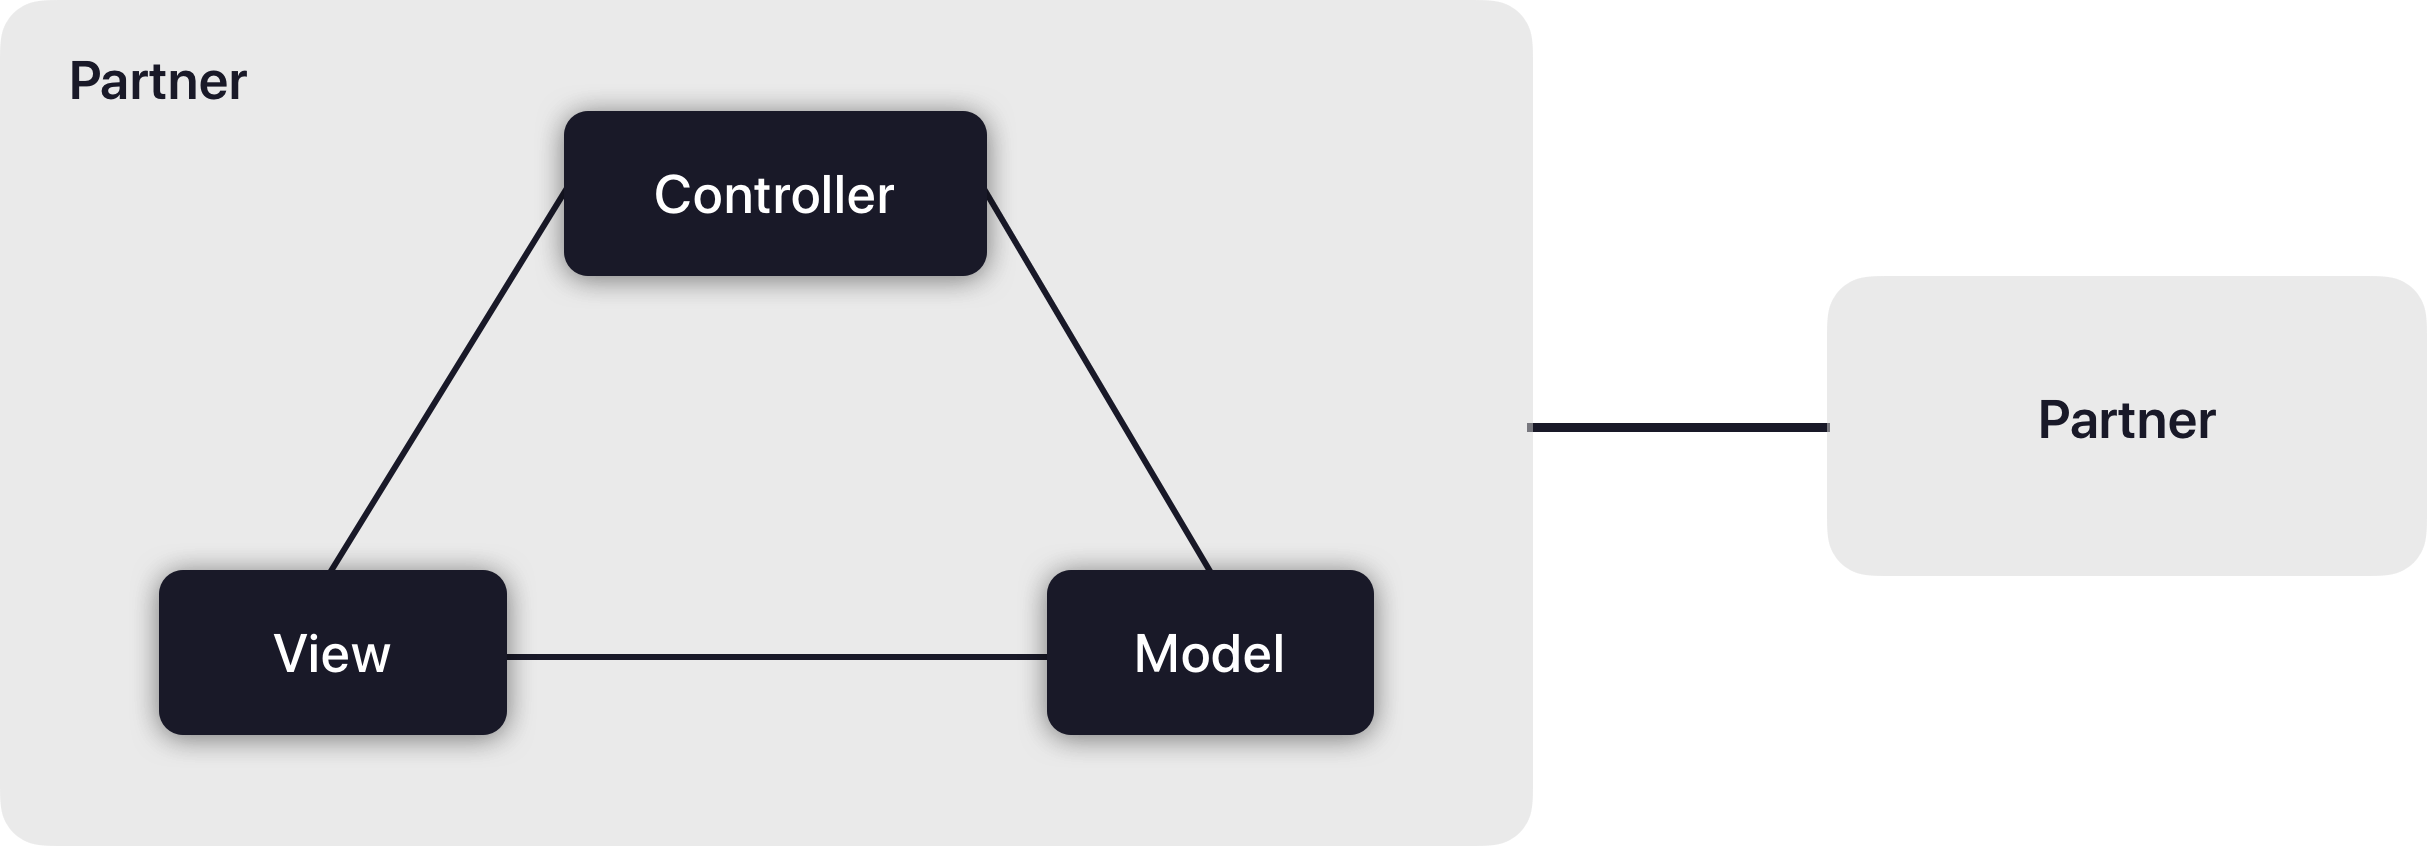
\includegraphics[width=1\textwidth]{graphics/Systemarchitektur}
  \caption{Schema der Systemarchitektur}
\end{figure}
Die Softwarearchitektur lässt sich auf zwei Ebenen betrachten, das Gesamtsystem mit der mobilen Anwendung des Patienten und der Desktopanwendung des Arztes oder einer weiteren mobilen Anwendung und die Teilsysteme auf den jeweiligen Geräten. \\\\
Da die einzelnen Geräte im Gesamtsystem gleichberechtigt miteinander kommunizieren sollen, wird es als Partnernetz realisiert.\\\\
Die Teilsysteme auf den Nutzergeräten enthalten lokale Daten, die in einer graphischen Benutzeroberfläche dargestellt werden sollen. Um die Datenverwaltung von der Darstellung zu trennen, wird die Model-View-Controller Architektur verwendet.
\printnoidxglossaries

% Abbildungsverzeichnis
\listoffigures
 
\end{document}